% PAKETE UND DOKUMENTKONFIGURATION
\documentclass[11pt, a4paper]{scrbook}

% Encoding für Umlaute
\usepackage[utf8]{inputenc}
\usepackage[T1]{fontenc}

% Silbentrennung
\usepackage[ngerman]{babel}

% erweiterte Matheumgebungen und Formelnummer mit Sectionnummer
\usepackage{amsmath}

% zusätzliche mathematische Schriftarten
\usepackage{amsfonts}

% verschiedene mathematische Symbole
\usepackage{amssymb}

%
\usepackage{textcomp}
\usepackage{mathtools}

% Einheiten setzen z.B. \SI{10}{\kilo\gram\meter\per\second\squared}
% Fehler: \SI{10 +- 0,2e-4}{\metre}
\usepackage{siunitx}
\sisetup{
  output-decimal-marker={,},
  separate-uncertainty
}

% Bilder einfügen
\usepackage{graphicx}

% Textfarbe
\usepackage[dvipsnames]{xcolor}

% Verweise innerhalb des Dokuments
\usepackage{hyperref}
\hypersetup{
	colorlinks = true,
	allcolors = {black}
}

\newcommand{\vnabla}{\vec{\nabla}}
\newcommand{\ve}{\vec{E}}
\newcommand{\vb}{\vec{B}}
\newcommand{\vh}{\vec{H}}
\newcommand{\vd}{\vec{D}}

\newcommand{\todo}[1]{{\textcolor{Green}{(#1)}}}

\title{Störkörpermessung an Beschleunigungsresonatoren}
\author{Christopher Deutsch}

\begin{document}
	\frontmatter
	\maketitle
	\tableofcontents
	
	\mainmatter
	
	\chapter{Einleitung}
	
	
	\chapter{Theorie}	
	\section{Hohlraumresonatoren}
	Ein Hohlraumresonator besteht aus einem evakuierten Hohlraum, welcher durch ein leitendes Material begrenzt wird.
	Die im Hohlraum propagierenden elektromagnetischen Wellen werden an den leitenden Wänden reflektiert und führen zur Ausbildung von stehenden elektromagnetischen Wellen im Resonatorinnenraum, welche unter anderem zur Beschleunigung von elektrisch geladenen Teilchen genutzt werden können.
	Aufgrund der Randbedingungen an der näherungsweise ideal leitenden Grenzfläche müssen die folgenden Anforderungen an das elektromagnetische Feld gestellt werden:
	\begin{align}
		E_\parallel = 0 \qquad \text{und} \qquad B_\perp = 0\text{,}
		\label{eq:randbedingung_leiter}
	\end{align}
	wobei $E_\parallel$ die Tangentialkomponente und $B_\perp$ die Normalkomponente des elektrischen bzw.\ magnetischen Feldes auf der Grenzfläche kennzeichnet.
	Die Lösung der \textsc{Maxwell}-Gleichungen unter Beachtung dieser Grenzbedingungen zeigt, dass in Abhängigkeit der Geometrie des Hohlraums, eine unbegrenzte Anzahl von Moden mit bestimmten Frequenzen im Resonator auftreten können.
	Die Klassifizierung der einzelnen Moden erfolgt dabei anhand ihrer Feldkonfiguration relativ zur Propagationsrichtung der hin- und rücklaufenden Wellen im Resonator.
	Dabei unterscheidet man zwischen transversal elektrischen (TE)-Moden, welche lediglich transversale elektrische und longitudinal magnetische Felder aufweisen und transversal magnetischen (TM)-Moden, bei denen der umgekehrte Fall eintritt.
	
	Viele der in Beschleunigern verwendeten Kavitäten\footnote{von lat.\ \emph{cavum} "Höhle": Hohlraumresonator oftmals engl. \emph{Cavity}} basieren auf kreiszylindrischen Resonatoren\footnote{engl. \emph{Pillbox-Cavities}, für deren Ähnlichkeit mit einer Tablettenschachtel}, welche eine analytische Lösung der \textsc{Maxwell}-Gleichungen erlauben.
	Daher soll im Folgenden die Feldkonfiguration der verschiedenen Moden am Beispiel der \emph{Pillbox-Cavity} (Abb. ???) dargestellt und die in dieser Arbeit verwendete Notation eingeführt werden.
	Dabei genügt die Betrachtung der longitudinalen Felder eines zylindrischen Hohlraums mit Radius~$R$ und Länge~$L$ in Zylinderkoordinaten $(r, \theta, z)$, da durch diese die transversalen Feldkomponenten eindeutig festgelegt sind \cite{hillert}.
	Man findet für die Moden in dem kreiszylindrischen Resonator \cite{wangler}:
	\begin{subequations}
		\begin{align}
		\mathrm{TM}_{mnp}\text{-Mode:} \quad E_z = E_0 J_m(k_{mn} r) \cos(m \theta) \cos\left(\frac{p \pi}{L}\right) \exp(i \omega_{mnp} t) \qquad B_z = 0\\
		\mathrm{TE}_{mnp}\text{-Mode:} \quad B_z = B_0 J_m(k_{mn}^\prime r) \cos(m \theta) \sin\left(\frac{p \pi}{L}\right) \exp(i \omega_{mnp}^\prime t) \qquad  E_z = 0
		\end{align}
		\label{eqs:felder_pillbox}
	\end{subequations}
	wobei die Konstante $k_{mn}^{(\prime)}$ definiert ist als:
	\begin{align}
	k_{mn}^{(\prime)} := \frac{x_{mn}^{(\prime)}}{R}
	\end{align}
	mit der $n$-ten positiven Nullstelle $x_{mn}$ Besselfunktion $m$-ter Ordnung $J_m(x)$ respektive ihrer Ableitung $J_m^\prime(x)$.
	Aus Gleichungen \eqref{eqs:felder_pillbox} folgt dann die Bedeutung der Indizes $m, n$ und $p$:
	Der Index $m$ ($m=0, 1, \dots$) beschreibt die Periodenzahl der Feldkomponente in azimutaler Richtung.
	Weiterhin wird durch $n$ ($n=1, 2, \dots$) die Anzahl der Knoten der longitudinalen Feldkomponente in radialer Richtung (ausgenommen Knoten im Ursprung mit $r=0$) gegeben.
	Schließlich gibt der Index $p$ (TM-Mode: $p= 0, 1, \dots$; TE-Mode: $p = 1, 2, \dots$) die Anzahl der halben Perioden in longitudinaler Richtung an.
	
	Die Kreisfrequenz~$\omega_{mnp}$ der einzelnen Moden ist dabei gegeben durch \cite{wangler}:
	\begin{align}
	\omega_{mnp}^{(\prime)} = c \cdot \sqrt{\left( k_{mn}^{(\prime)}\right)^2 + \left( \frac{p \pi z}{L} \right)^2}
	\end{align}
	\todo{Bilder Pillbox, Felder und TM010 im Beschleuniger}
	
	Eine analytische Berechnung der Moden von komplexeren Resonatorgeometrien ist nicht mehr möglich und es muss auf numerische Methoden zurückgegriffen werden.
	Dazu wird in dieser Arbeit \emph{CST Microwave Studio\textsuperscript{\textregistered}} verwendet, welches die Lösung der Maxwell-Gleichungen diskretisiert und auf ein Eigenwertproblem zurückführt.
	
	\section{Hohlraumresonatoren2}
	\begin{figure}[h]
		\centering
		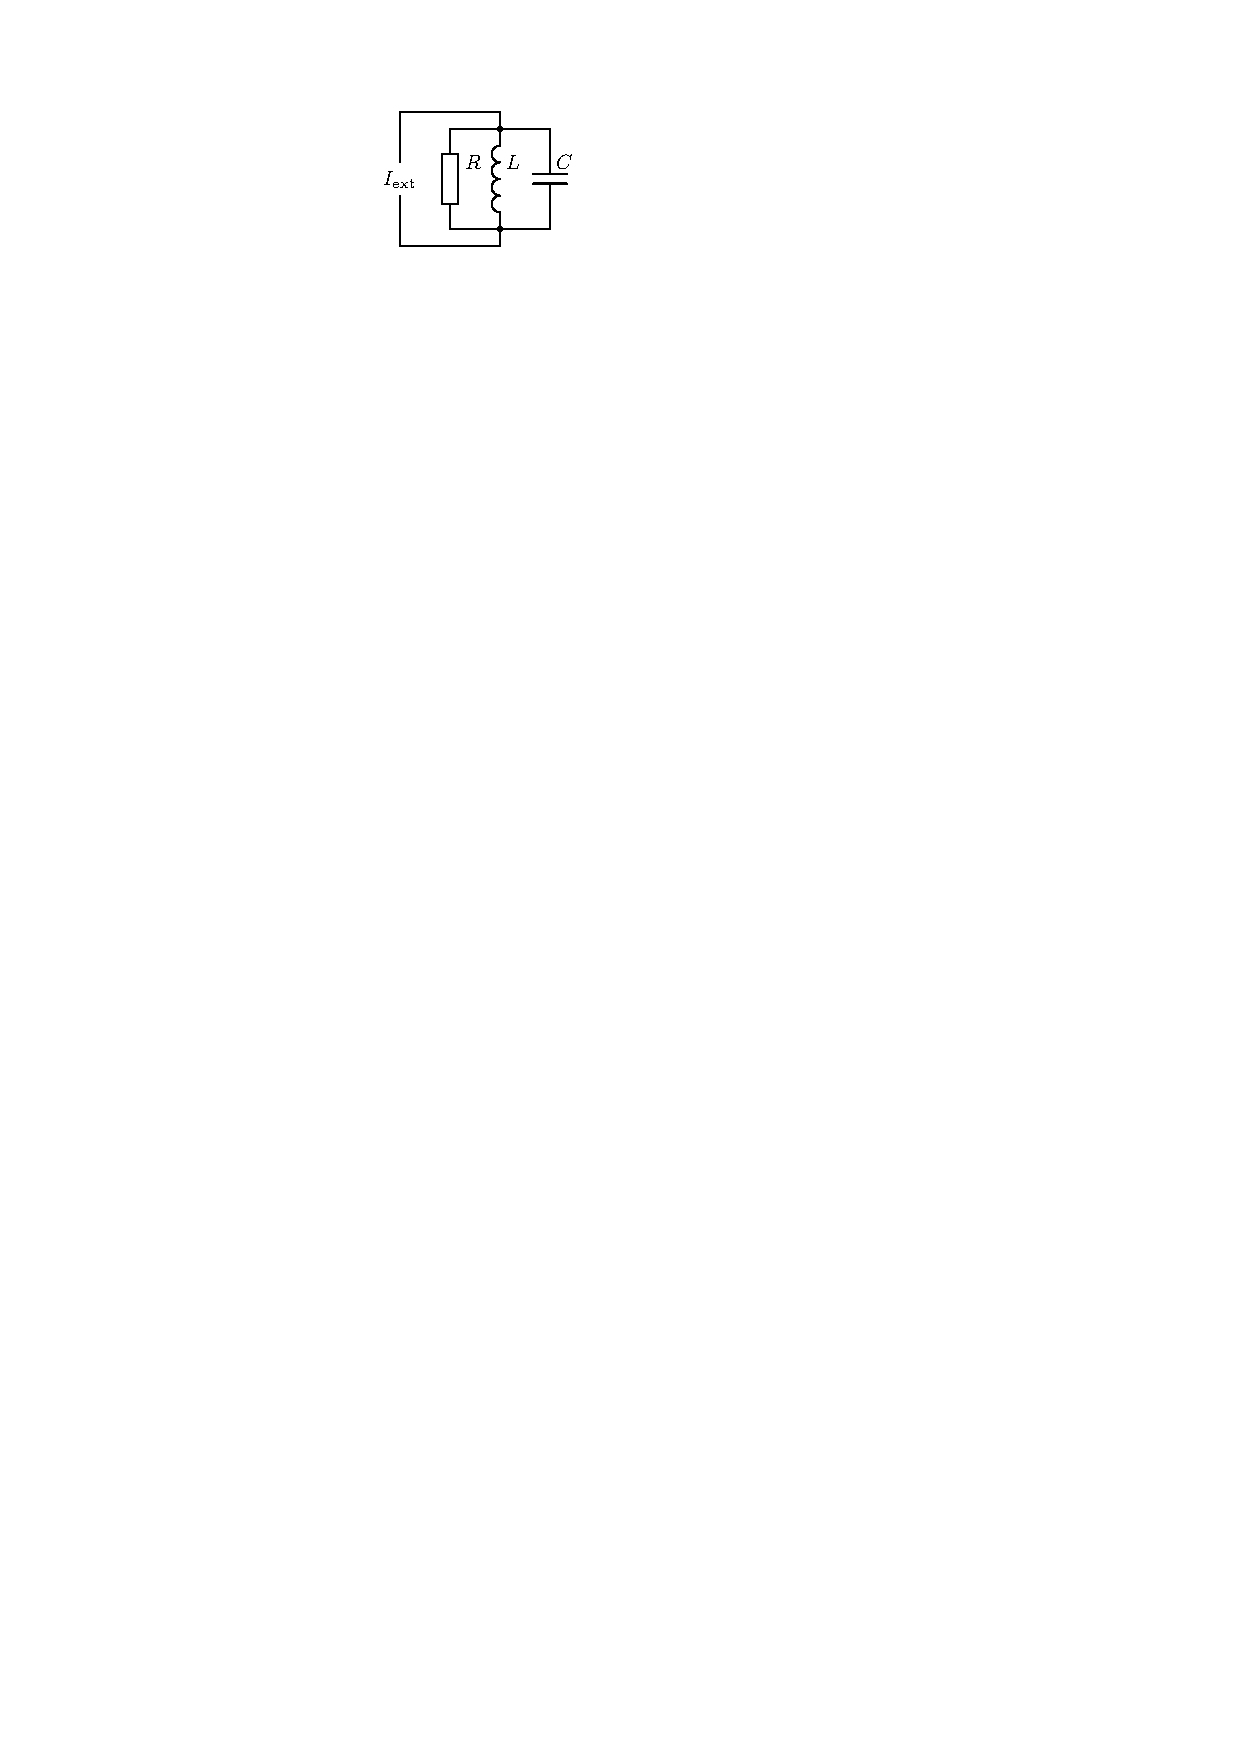
\includegraphics[width=0.35\textwidth]{./figures/RLC_circuit.pdf}
		\caption{RLC Parallelschwingkreis}
		\label{fig:rlc_circuit}
	\end{figure}
	Die elektrischen Eigenschaften von Hohlraumresonatoren in der Nähe einer Resonanz können durch das Modell des Parallelschwingkreises erklärt werden.
	Zur vollständigen Beschreibung ist die Angabe der drei Kenngrößen: Widerstand~$R$, Induktivität~$L$ und Kapazität~$C$ ausreichend.
	Für die Behandlung von Kavitäten ist es zweckmäßig andere Parameter zur Beschreibung zu verwenden.
	Dazu verwendet man die Eigenfrequenz~$\omega_0$, Kreisgüte~$Q_0$ und Widerstand~$R$ des Schwingkreises.
	Die Eigenfrequenz des Kreises folgt aus der \textsc{Thomson}schen Schwingungsgleichung:
	\begin{align}
		\omega_0 = \frac{1}{\sqrt{L C}}
	\end{align}
	und die Kreisgüte aus ihrer Definition:
	\begin{align}
		Q_0 &\coloneqq 2\pi \cdot \frac{\text{gespeicherte Energie}}{\text{Energieverlust pro Periode}} = \omega_0 R C
	\end{align}
	Nach der Einführung dieser Kenngrößen kann die Impedanz des Kreises beziehungsweise des Hohlraumresonators ausgedrückt werden als:
	\begin{align}
		Z(\omega) = \frac{R}{1 + i Q_0 \left( \frac{\omega}{\omega_0}  - \frac{\omega_0}{\omega}\right)}
	\end{align}
	
	Bisher war die Betrachtung auf ungetriebene Resonatoren beschränkt und soll nun auf die Anregung durch ein externes Hochfrequenzsignal erweitert werden.
	Zur Übertragung der Leistung aus einem Wellenleiter mit charakteristischer Impedanz $Z_0$ in eine Schwingungsmode der Kavität können verschiedene Methoden verwendet werden.
	Eine ist die induktive Kopplung an das Magnetfeld der Mode, bei der der Wellenleiter mit einer Leiterschleife (die sog.\ Koppelschleife) im Resonator verbunden ist.
	Dadurch wird in der Leiterschleife ein hochfrequenter Wechselstrom angeregt, welcher wiederum ein Magnetfeld erzeugt, dass Moden in der Kavität resonant anregen kann\footnote{Dies ist nur möglich wenn die jeweilige Mode am Ort der Koppelschleife ein nicht verschwindendes Magnetfeld besitzt.}.
	
	Im Modell des Parallelschwingkreises bedeutet dies, dass die Impedanz~$Z(\omega)$ der Kavität durch die induktive Kopplung transformiert wird.
	Direkt hinter der Koppelschleife habe der Resonator die transformierte\footnote{insbesondere gilt: $Z^\prime(\omega) \propto Z(\omega)$ \todo{Hier}} Impedanz $Z^\prime(\omega)$.
	Man definiert als Maß für die Kopplung den sog.\ Koppelfaktor:
	\begin{align}
		\kappa = \frac{Z^\prime(\omega_0)}{Z_0}
		\label{eq:koppelfaktor}
	\end{align}
	mit dem Wellenwiderstand~$Z_0$ des Wellenleiters.
	Man unterscheidet zwischen unterkritischer $(\kappa < 1)$, kritischer $(\kappa = 1)$ und überkritischer Kopplung $(\kappa > 1)$.
	Im Falle von resonanter Anregung bei kritischer Kopplung folgert man aus Gleichung \eqref{eq:koppelfaktor}, dass der Wellenleiter mit seiner charakteristischen Impedanz abgeschlossen ist und somit keine Reflexionen an der Koppelschleife entstehen.
	Dies ist für den Betrieb von Beschleunigungsresonatoren wünschenswert, da dadurch die gesamte Leistung in den Resonators transmittiert wird\todo{weg?}.
	
	Von besonderem Interesse ist der komplexe Reflexionskoeffizient $\rho$, da dieser direkt mit einem vektoriellen Netzwerkanalysator messbar ist.
	Er beschreibt das Verhältnis der komplexen Spannungsamplituden von hin- und rücklaufender Welle in einem Wellenleiter.
	Aus der Leitungstheorie \cite{pozar} folgt für den Reflexionskoeffizienten am Übergang von einem Wellenleiter mit Wellenwiderstand $Z_0$ auf eine Abschlussimpedanz $Z^\prime$:
	\begin{align}
		\rho = \frac{U_{-}}{U_{+}} = \frac{Z^\prime - Z_0}{Z^\prime + Z_0}
	\end{align}
	
	
	\todo{Hier weiter}
	Ebenfalls wird die zusätzliche Impedanz des Leiters in den Resonator transformiert, was die Güte des Gesamtsystems verändert:
	\begin{align}
		\frac{1}{Q} = \frac{1}{Q_0} + \frac{1}{Q_\mathrm{ext}} \\
		Q_0 = (1 + \kappa) \cdot Q
	\end{align}
	Im folgenden ist der komplexe Reflexionsfaktor $\rho$ von besonderem Interesse:

	Es folgt für den Reflexionsfaktor
	\begin{align}
		\rho(\omega) = \frac{(\kappa - 1) + i  Q_0 \left( \frac{\omega}{\omega_0}  - \frac{\omega_0}{\omega}\right)}{\left( \kappa + 1 \right) + i  Q_0 \left( \frac{\omega}{\omega_0}  - \frac{\omega_0}{\omega}\right)}
	\end{align}
	Mit dem Betrag:
	\begin{align}
		| \rho(\omega) | = \sqrt{\frac{(\kappa - 1)^2 + Q_0^2 \left( \frac{\omega}{\omega_0}  - \frac{\omega_0}{\omega}\right)^2}{(\kappa + 1)^2 + Q_0^2 \left( \frac{\omega}{\omega_0}  - \frac{\omega_0}{\omega}\right)^2}}
	\end{align}
	Damit ist die vom Resonator aufgenommene Leistung:
	\begin{align}
		P_\mathrm{a} = P_0 (1- |\rho|^2)
	\end{align}
	\section{Resonante Störkörpermessung}
	Feld der ungestörten Cavity $\ve_0$ und der gestörten $\ve_1$:
	\begin{subequations}
		\begin{align}
		&\ve_{0,1}(x,y,z,t) = \ve_{0,1}(x,y,z) \, e^{i \omega t} \\
		&\vh_{0,1}(x,y,z,t) = \vh_{0,1}(x,y,z) \, e^{i \omega t}
		\end{align}
	\end{subequations}
	wobei im folgenden mit nur mit den komplexen Amplituden gerechnet wird.
	Mit den Maxwell-Gleichungen:
	\begin{subequations}
		\begin{align}
			&\vnabla \times \ve = - \frac{\partial \vb}{\partial t} \\
			&\vnabla \times \vh = \frac{\partial \vd}{\partial t}
		\end{align}
	\end{subequations}
	folgt nach Elimination der Zeitabhängigkeit:
	\begin{subequations}
		\begin{align}
			&\vnabla \times \ve_{0,1} = - i \omega_{0,1} \vb_{0,1} \\
			&\vnabla \times \vh_{0,1} = i \omega_{0,1} \vd_{0,1}
		\end{align}
	\end{subequations}
	Unter der Verwendung dieser zeitunabhängigen Gleichungen bildet man:
	\begin{align}
	\vnabla \cdot \left( \ve_0^* \times \vh_1\right) &= \vh_1 \cdot \left( \vnabla \times \ve_0^* \right) - \ve_0^* \cdot \left( \vnabla \times \vh_1 \right) \nonumber \\
	&= i \omega_0 \vb_0^* \vh_1 - i \omega_1 \ve_0^* \vd_1 \label{eq:e0h1}
	\end{align}
	und
	\begin{align}
		\vnabla \cdot \left( \ve_1 \times \vh_0^* \right) &= \vh_0^* \cdot \left( \vnabla \times \ve_1 \right) - \ve_1 \cdot \left( \vnabla \times \vh_0^* \right) \nonumber \\
		&= i \omega_0 \ve_1 \vd_0^* - i \omega_1 \vb_1 \vh_0^* \label{eq:e1h0}
	\end{align}
	Anschließend führt man die Integration über das Resonatorvolumen $V$ durch:
	\begin{align}
		\int_{V} \mathrm{d}V \left[ \vnabla \cdot \left( \ve_0^* \times \vh_1 + \ve_1 \times \vh_0^* \right) \right] = \int_{\partial V} \mathrm{d}S \left[ \vec{n} \cdot \left( \ve_0^* \times \vh_1 + \ve_1 \times \vh_0^* \right)\right] \label{eq:volint}
	\end{align}
	Aufgrund der Randbedingungen am leitenden Material des Resonators gilt $\ve \times \vh \perp \vec{n}$ und somit ist die verschwindet die rechte Seite von Gleichung \eqref{eq:volint} folgt nach Einsetzen der Relationen \eqref{eq:e0h1} und \eqref{eq:e1h0}:
	\begin{align}
		\omega_0 \int_{V} \mathrm{d}V \left( \vb_0^* \cdot \vh_1 + \ve_1 \cdot \vd_0^* \right) = \omega_1 \int_{V} \mathrm{d}V \left( \vb_1 \cdot \vh_0^* + \ve_0^* \cdot \vd_1 \right)
	\end{align}
	Nach Umformung folgt:
	\begin{align}
		\frac{\omega_1 - \omega_0}{\omega_0} = \frac{\int_{V} \mathrm{d}V \left[ \left( \vb_0^* \cdot \vh_1 - \vb_1 \cdot \vh_0^* \right) + \left( \ve_0^* \cdot \vd_1 - \ve_0^* \cdot \vd_1 \right)\right]}{\int_V \mathrm{d}V \left[ \vb_1 \cdot \vh_0^* + \ve_0^* \cdot \vd_1 \right] }
	\end{align}
	Unter der Verwendung von:
	\begin{subequations}
		\begin{align}
			&\vd = \epsilon_0 \ve + \vec{P} \\
			&\vh = \frac{1}{\mu_0} \vb - \vec{M}
		\end{align}
	\end{subequations}
	folgt die Slater-Formel?:
	\begin{align}
		\frac{\omega_1 - \omega_0}{\omega_0} = - \frac{\int_V \mathrm{d}V \left[ \vb_0^* \cdot \vec{M} + \ve_0^* \cdot \vec{P} \right]}{\int_V \mathrm{d}V \left[ \vb_1 \cdot \vh_0^* + \ve_0^* \cdot \vd_1 \right]}
	\end{align}
	Da der Störkörper die Energie des Resonators kaum beeinflusst, kann im Nenner das gestörte Feld durch das ungestörte genähert werden und man erhält:
	\begin{align}
		\frac{\omega_1 - \omega_0}{\omega_0} = - \frac{\int_V \mathrm{d}V \left[ \vb_0^* \cdot \vec{M} + \ve_0^* \cdot \vec{P} \right]}{4 W_0}
	\end{align}
	wobei $W_0 = \int_V w_\mathrm{em} \, \mathrm{d}V = \int_V \frac{1}{2} (\ve \cdot \vd + \vb \cdot \vh) \, \mathrm{d}V$ die Energie des elektromagnetischen Feldes im Resonator ist. NEIN VIERFACHE ENERGIE.
	Im Rahmen dieser Bachelorarbeit wird eine dielektrische Kugel verwendet $\vec{M} = 0$, welche klein gegen die Dimensionen des Resonators ist. Für die Polarisation folgt (Jackson S.\ 115) unter der Annahme eines homogenen Feldes:
	\begin{align}
		\vec{P} = 3 \frac{\epsilon_\mathrm{r} - 1}{\epsilon_\mathrm{r} + 2} \epsilon_0 \ve_0
	\end{align}
	und damit:
	\begin{align}
		\frac{\omega_1 - \omega_0}{\omega_0} = - 3 \left( \frac{\epsilon_\mathrm{r} - 1}{\epsilon_\mathrm{r} + 2} \right) \epsilon_0 V_\mathrm{s} \frac{|\ve_0|^2}{4 W_0}
	\end{align}
	\begin{align}
		\alpha_\mathrm{s} = 3 \left( \frac{\epsilon_\mathrm{r} - 1}{\epsilon_\mathrm{r} + 2} \right) \epsilon_0 V_\mathrm{s}
	\end{align}
	\begin{align}
		\frac{\Delta \omega}{\omega_0} = \frac{\omega_0 - \omega_1}{\omega_0} = \alpha_\mathrm{s} \cdot \frac{|\ve|^2}{4 W_0}
	\end{align}
	\begin{align}
		|\ve| = \sqrt{4 \cdot \frac{W_0}{\alpha_\mathrm{s}} \cdot \frac{\Delta \omega}{\omega_0}}
	\end{align}
	Ist die unbelastete Güte des Resonators bekannt, so kann das elektrische Feld in Abhängigkeit der Verlustleistung des Resonators geschrieben werden als:
	\begin{align}
		\frac{|E_0|}{\sqrt{P_\mathrm{V}}} = \sqrt{4 \frac{Q_0}{\alpha_s} \frac{\Delta \omega}{\omega_0^2}}
	\end{align}
	
	
	\chapter{Störkörpermessung}
	
	\chapter{Fazit}
	
	\backmatter
		
	\begin{thebibliography}{19}
	\bibitem{hillert}
		\textsc{W.\ Hillert},
		\emph{E 106: Cavities, Details on the experimental method}, Bonn, 2008.

	\bibitem{wangler}
		\textsc{T.\ P.\ Wangler},
		\emph{Principles of RF Linear Accelerators},
		Wiley, New York, 1998.
	
	\bibitem{pozar}
		\textsc{D.\ M.\ Pozar},
		\emph{Microwave Engineering}, 4th ed.,
		Wiley, New York, 2011.
	
	\bibitem{jackson}
		\textsc{J.\ D.\ Jackson},
		\emph{Classical Electrodynamics}, 1st ed.,
		Wiley, New York, 1962.
	
	\end{thebibliography}
	
	\chapter{Danksagung}
	
	\listoffigures
	\listoftables
	
\end{document}
